% ITEX root = ../Thesis.tex

In this project, published data was provided on multiple experiments on microbial population and growth.Growth conditions including medium and temperature were manipulated and populations were recorded through different measurements techniques such CFU, or OD595. The Population numbers and time were recorded discretely at different time intervals. The data were stored in a \textit{.csv} file, \textit{LogisticGrowthData.csv}. All four mechanistic models were fitted on the data.

\subsection{Computing Tools}
\textit{Python}

Python software was used to wrangle the data. The data provided was in one large \textit{.csv} file and needed to be manipulated before being filtered. Combination of functions and commands were used to wrangle the data and remove unwanted data points, as well as converting to log space. \textit{Pandas} and \textit{Numpy} were the two packages used for the purpose of data import and carrying out mathematical manipulations of the data set.

\textit{R}

R software was used to filter the data set and carry out data analysis. Software package \textit{dplyr} was used to filter the data set and create unique ID’s, which were saved as \textit{.rda} files. The mechanistic equations to be fitted on the data and functions to find optimal starting value for the parameters were done in R. Using \textit{minpack.lm} package, non-linear regression analysis was carried out using the \textit{nlsLM()} function as well as plotting the different unique analysis. The package BisRNA was used to perform fisher's method to get a p-value statistic from multiple independent tests for the linear regression of growth rate and temperature. The \textit{stringr} package was used for setting wrappers and filtering the unique species by their string. Lastly, gridExtra package was used to save tables from R in pdf format.

\textit{Bash}

Bash script was used to run the python, R scripts and the latex file, to convert the latex into a pdf.

\subsection{Data Exploration and Filtering}

The data was first wrangled before being filtered. All abundance recordings of OD595 were first multiplied by 100. Next the data was treated in linear scale, therefore negative time and population values were either removed or shifted. In addition, negative time values were set to zero as it is not realistic to have a negative time recordings. The data was then transformed to a log scale, by taking the common logarithm of the population abundance. This is to fit the criteria of three of the models and make the data less skewed. Although the Logistic model is not in log scale, the output value is of the function is, to maintain the linearity of the function, and interpret the paramters biologically.

Data was then filtered based on the headings: species, medium, temperature, citation and replicate. It is important to note that method of collecting population count was not a factor in the model fitting and assessing of best model(s). The unique data sets were saved in .rda files which included the unique ID’s and a data frame of the time intervals, labelled Time and the common logarithm of the population count at each discrete time interval, labelled Abundance.

The four mechanistic models were then fitted to all the different sub-data sets. Of the four, the Logistic formula is derived from bacterial growth properties, where $r_{max}$ is the maximum growth rate during the exponential phase and $N_{max}$ represents the carrying capacity, while the other three models are based on mathematical derivations. However, since all the models utilise the same parameters, their values can be interpreted to have the same biological interpretations (Levins 1996). Using R Programming Language, each of the models will be tested on the data and the Akaike Information Criterion (AIC) will be the statistic to analyse the model of best fit.

\subsection{Fitting the models}

The R software will be used to test the models and their fits. Using the package minpack.lm, the nlsLM() function is used to fit the non-linear mechanistic models. Since it is non-linear regression fitting, parameter starting values must be estimated within range of the global maximum or minimum respectively as unlike linear regression, the function can find an optimal value, but only be a local rather than a global minimum or maximum. To fit the Baranyi, Gompertz and Buchanan models, it requires inputting four starting parameter values ($N_0$, $t_lag$, $r_{max}$, $N_{max}$) for the parameters of the equation, while the Logistic model only requires three of the parameters, not including $t_lag$.

\subsection{Finding Parameters}

$N_0$ is the starting population value at the first-time recording, thus the first data point. The carrying capacity ($N_{max}$) is the largest value found in the data set, which is the maximum value of the data set. The growth rate, $r_{max}$, is the largest gradient value of the derivative found at the point $\frac{N_{max}}{2}$, otherwise known as the inflection point. To find the estimate of this parameter, a function utilising a while loop was used. It describes the rate of change of the population over time, given the equation below:
\begin{equation*}
    \frac{dx}{dt}=\frac{x_{t+1}-x_{t}}{(t+1)-t}\label{eq:slope} \tag{4}
\end{equation*}
where $dx$ represents the change in population count from time $t$ to $t+1$. Starting from the first data point and progressing to the final two data points, each iteration calculated the slope between adjacent data points, saving all results in a vector and the largest value was taken to be the $r_max$.

The models include a time lag, which is a delay in time of bacteria growth. The estimation is found through the intersection between the lag phase, which can be represented by the starting population value, and exponential growth phase, represented by the slope of the growth rate \cite{peleg2011microbial}. This was calculated by the intersection of y=$N_0$ and the line with gradient $r_{max}$. Using the y-intercept ($y_{int}$) value from the $r_{max}$ line that produced the greatest slope, rearranging of the linear equation leads to the formula:
\begin{equation*}
   t_lag=\frac{N_0 - y_{int}}{r}
\end{equation*}
Figure 1 below shows an example of this derivation.
\begin{figure}[h]
\centering
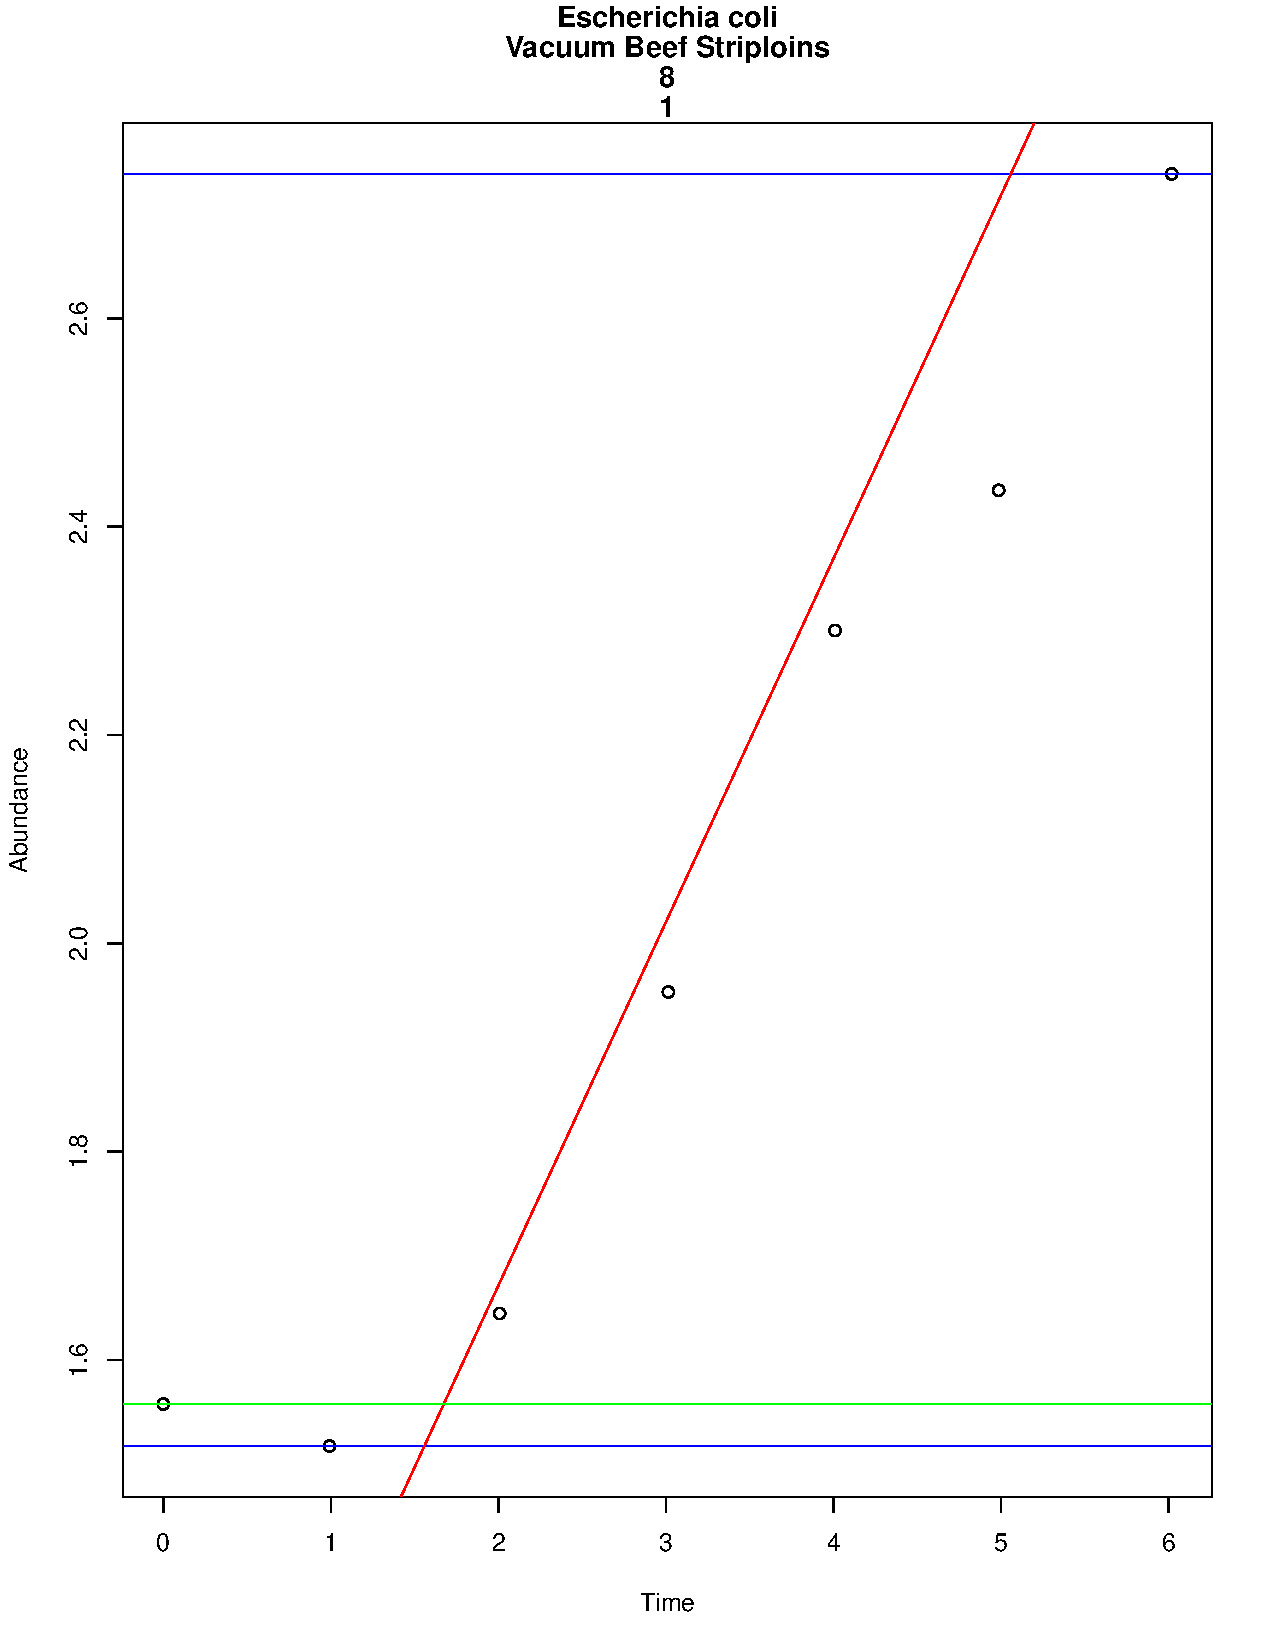
\includegraphics[scale=0.5]{../Results/Parameters_Ecoli.pdf}
\caption{The first replicate of species Escherichia coli grown in medium of Vacuum Beef Striploin at a temperature of 8\degree C. The blue lines represent $N_0$ (lower blue line) and $N_{max}$ (upper blue line). The red line represents the slope representing $r_{max}$. Finally the green line is the estimate of the $t_{lag}$, where x-value of the intersection of the red and green is the parameter estimate.}
\label{fig:Starting parameters}
\end{figure}

Species and medium were the factors accounted for when identifying the correlation between temperature and growth rate. For each of the unique ID’s, the growth rates, temperatures, Species and growth medium were recorded in a large matrix. The matrix was subset to the different unique ID’s and linear regression analysis was done to analyse the correlation.

\subsection{Fitting Analysis}

All models were fitted on all of the data and the best fits were analysed using the Akaike Information Criterion (AIC), which measures the amount of lost information when fitting the models \cite{posada2004model}. We are using AIC to assess the model fit as it is able to analyse nested and non-nested model fits as well as being less penalising for additional parameters unlike BIC \cite{posada2004model}. In this case, the four mechanistic models which all have similar parameters with $t_{lag}$ being the additional parameter.

\subsection{Additional investigation}

Aside from identifying the best fit model, another aspect being investigated is the correlation between growth rate and temperature. The models used despite their derivations contain the same parameters, having a unified theory for the bacterial growth behaviour \cite{levins1966strategy}. Investigating how the growth rate changes as temperature increases through linear regression for each of the unique species and mediums will give insight if the trends are similar. A linear regression was compared to the formula found in the paper of \textit{Ratkowsky et al.} The correlation coefficients from the linear regression and p-values of the slope coefficients were recorded and saved in a table.
